\chapter{Results}
\label{ch:results}

%-------------------------------------------------------

% TODO: opening paragraph. Name the input video, its resolution, frame
% rate and length, and state which settings each screenshot below uses.
% Assignment requirement: "Include samples of outputs of your program."

%%%%%%%%%%%%%%%%%%%%%%%%%%%%%%%%%%%%%%%%%%%%%%%%%%%%%
\section{Input Video}
\label{sec:input}
%%%%%%%%%%%%%%%%%%%%%%%%%%%%%%%%%%%%%%%%%%%%%%%%%%%%%

\begin{table}[h]
    \centering
    \caption[Input video properties.]%
    {Properties of the input video used for all results in this chapter.}

    \begin{tabular}{P{2.2in}|P{2.2in}}
        \specialrule{1.5pt}{0pt}{0pt}
        Property & Value \\
        \hline\hline
        File name & \texttt{barriers.avi} \\
        \specialrule{0.5pt}{0pt}{0pt}
        Resolution (W $\times$ H) & $640 \times 480$ \\
        \specialrule{0.5pt}{0pt}{0pt}
        Frame rate & 50 fps \\
        \specialrule{0.5pt}{0pt}{0pt}
        Frame count & 399 \\
        \specialrule{0.5pt}{0pt}{0pt}
        Duration & $\approx 8.0$ s \\
        \specialrule{0.5pt}{0pt}{0pt}
        Codec / container & FMP4 / AVI \\
        \specialrule{1.5pt}{0pt}{0pt}
    \end{tabular}
    \label{table:inputvideo}
\end{table}


%%%%%%%%%%%%%%%%%%%%%%%%%%%%%%%%%%%%%%%%%%%%%%%%%%%%%
\section{Main Window at Default Settings}
\label{sec:res-default}
%%%%%%%%%%%%%%%%%%%%%%%%%%%%%%%%%%%%%%%%%%%%%%%%%%%%%

% Covers Tasks 1-4: both videos and both histograms visible at once.
% TODO: describe what the screenshot shows and why the two histograms
% are identical at default settings.

\begin{figure}[H]
    \centering
    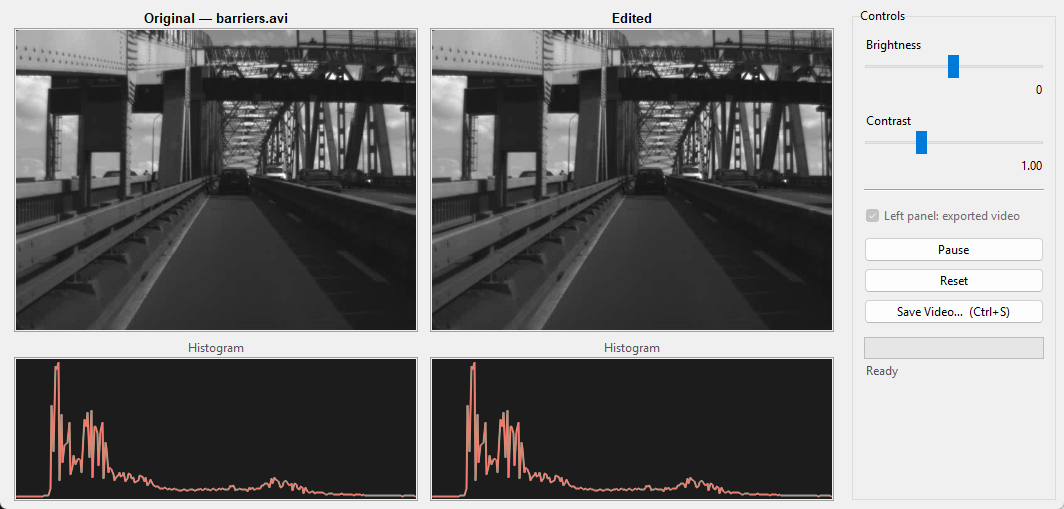
\includegraphics[width = \textwidth]{screenshot_default.png}
    \caption[Main window at default settings.]%
    {Full application window at the default settings ($\beta=0$,
    $\alpha=1.0$): the original video (left) and the preview video
    (right) with their respective histograms underneath, plus the
    control panel.}
    \label{fig:default}
\end{figure}


%%%%%%%%%%%%%%%%%%%%%%%%%%%%%%%%%%%%%%%%%%%%%%%%%%%%%
\section{Effect of the Brightness Control}
\label{sec:res-brightness}
%%%%%%%%%%%%%%%%%%%%%%%%%%%%%%%%%%%%%%%%%%%%%%%%%%%%%

% Covers Task 6 (brightness half).
% TODO: state the slider value used in each subfigure and describe the
% shift of the histogram, including any clipping.

\begin{figure}[H]
    \centering
    \begin{subfigure}{0.48\linewidth}
        \centering
        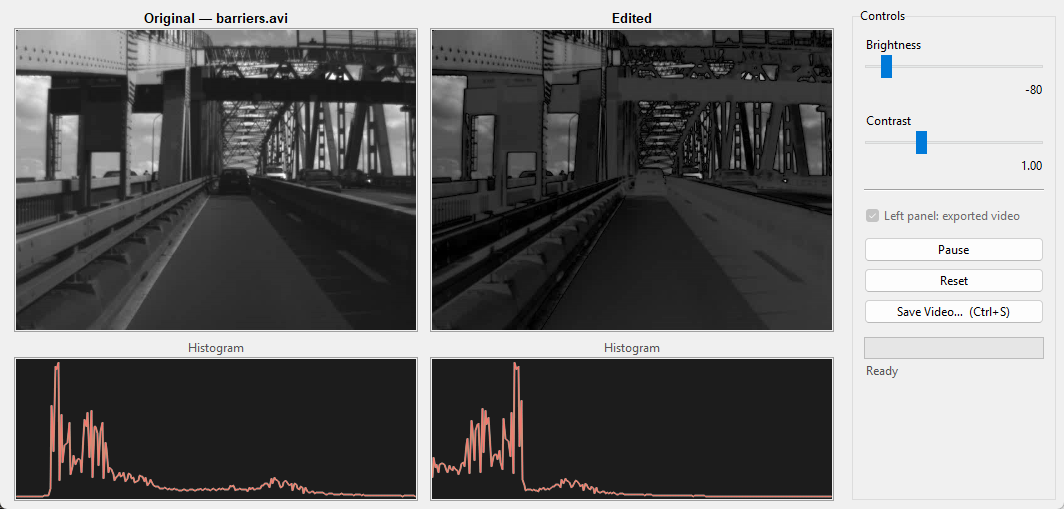
\includegraphics[width=\textwidth]{screenshot_brightness_low.png}
        \caption{$\beta = -80$}
        \label{fig:bright-low}
    \end{subfigure}
    \hfill
    \begin{subfigure}{0.48\linewidth}
        \centering
        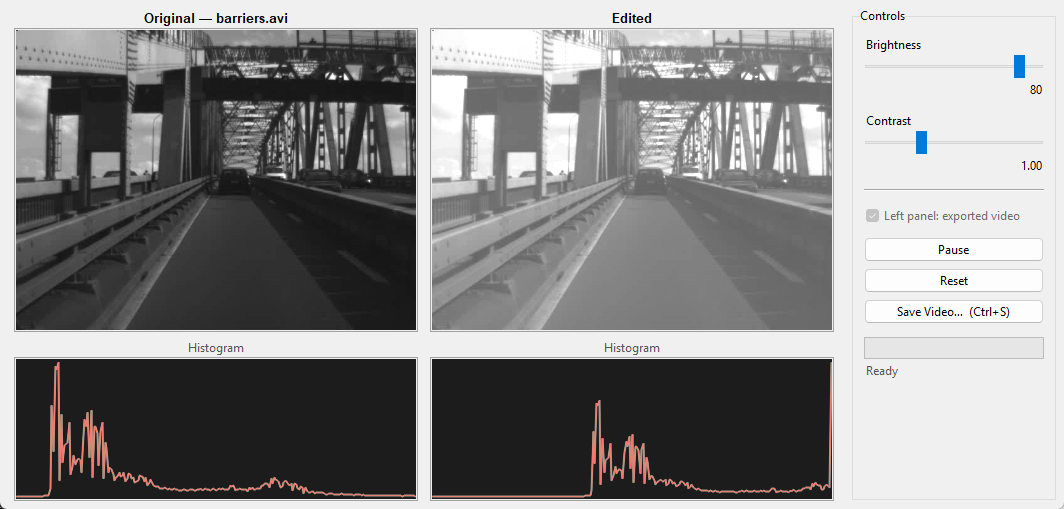
\includegraphics[width=\textwidth]{screenshot_brightness_high.png}
        \caption{$\beta = +80$}
        \label{fig:bright-high}
    \end{subfigure}
    \caption[Effect of the brightness control.]%
    {Preview video and its histogram at two brightness settings
    ($\alpha=1.0$ fixed in both), compared against the unmodified
    original on the left of each panel. The histogram translates left
    for negative $\beta$ and right for positive $\beta$, exactly as
    described in Table \ref{table:controls}.}
    \label{fig:brightness}
\end{figure}


%%%%%%%%%%%%%%%%%%%%%%%%%%%%%%%%%%%%%%%%%%%%%%%%%%%%%
\section{Effect of the Contrast Control}
\label{sec:res-contrast}
%%%%%%%%%%%%%%%%%%%%%%%%%%%%%%%%%%%%%%%%%%%%%%%%%%%%%

% Covers Task 6 (contrast half).
% TODO: state the slider value used in each subfigure and describe the
% stretching or compression of the histogram.

\begin{figure}[H]
    \centering
    \begin{subfigure}{0.48\linewidth}
        \centering
        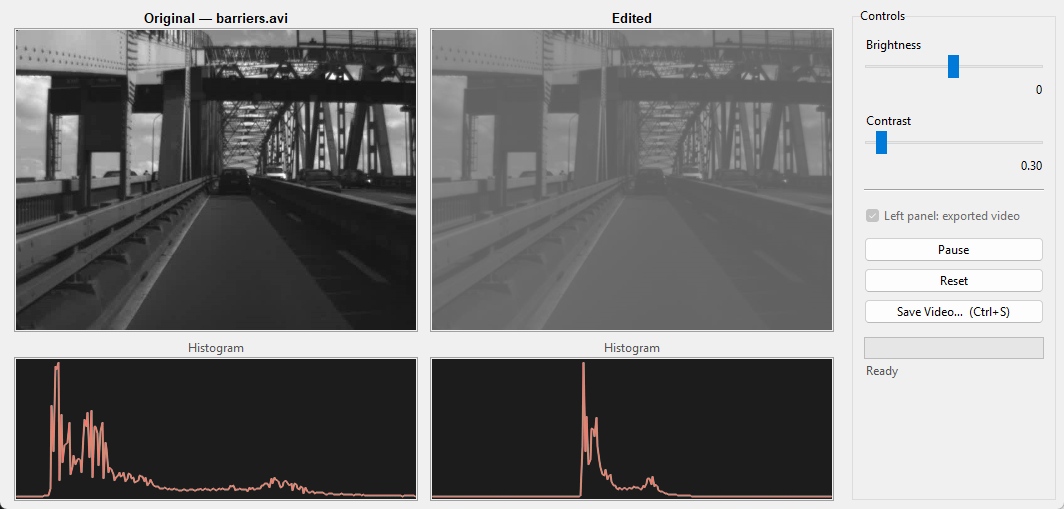
\includegraphics[width=\textwidth]{screenshot_contrast_low.png}
        \caption{$\alpha = 0.3$}
        \label{fig:contrast-low}
    \end{subfigure}
    \hfill
    \begin{subfigure}{0.48\linewidth}
        \centering
        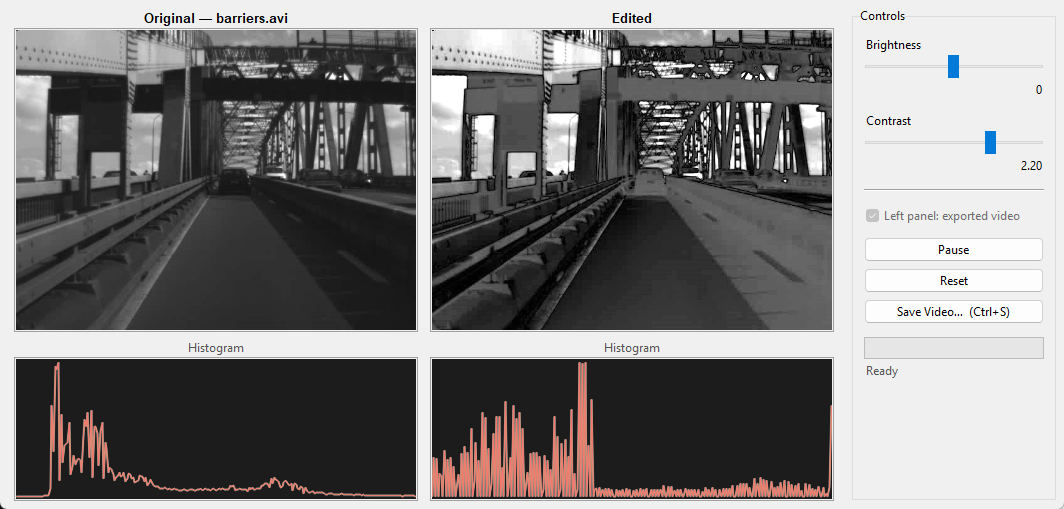
\includegraphics[width=\textwidth]{screenshot_contrast_high.png}
        \caption{$\alpha = 2.2$}
        \label{fig:contrast-high}
    \end{subfigure}
    \caption[Effect of the contrast control.]%
    {Preview video and its histogram at two contrast settings
    ($\beta=0$ fixed in both), compared against the unmodified
    original on the left of each panel. At $\alpha=0.3$ the histogram
    compresses toward mid-gray; at $\alpha=2.2$ it spreads out and
    several bins clip at 0 and 255.}
    \label{fig:contrast}
\end{figure}


%%%%%%%%%%%%%%%%%%%%%%%%%%%%%%%%%%%%%%%%%%%%%%%%%%%%%
\section{Continuous Playback}
\label{sec:res-loop}
%%%%%%%%%%%%%%%%%%%%%%%%%%%%%%%%%%%%%%%%%%%%%%%%%%%%%

% Covers Task 5.
% TODO: show the last frame and the restarted first frame, or describe
% how looping was verified.

\begin{figure}[H]
    \centering
    \begin{subfigure}{0.48\linewidth}
        \centering
        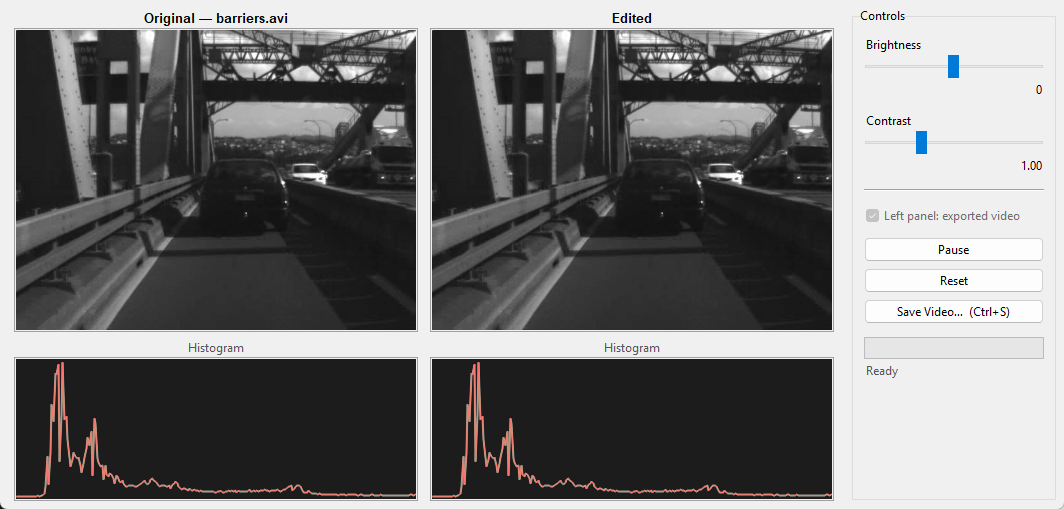
\includegraphics[width=\textwidth]{screenshot_loop_last.png}
        \caption{Frame 399 (final frame)}
        \label{fig:loop-last}
    \end{subfigure}
    \hfill
    \begin{subfigure}{0.48\linewidth}
        \centering
        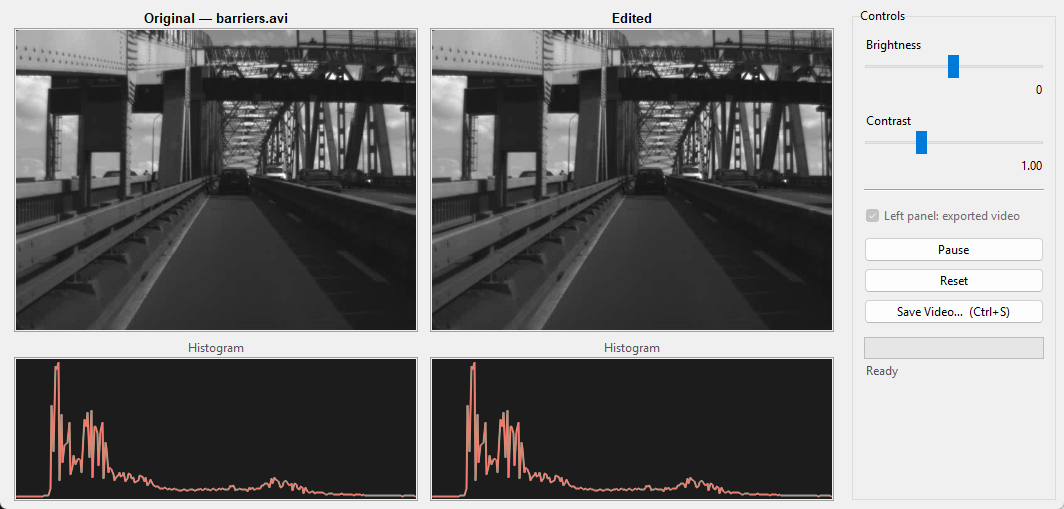
\includegraphics[width=\textwidth]{screenshot_loop_first.png}
        \caption{Frame 1, immediately after the automatic restart}
        \label{fig:loop-first}
    \end{subfigure}
    \caption[Automatic restart at end of stream.]%
    {Playback wrapping from the final frame of \texttt{barriers.avi}
    back to frame 1 without any user action, exercising the same
    end-of-stream/rewind path (\texttt{\_read\_looping}, Listing
    \ref{lst:task5-read}) shown in Section \ref{sec:task5}.}
    \label{fig:looping}
\end{figure}


%%%%%%%%%%%%%%%%%%%%%%%%%%%%%%%%%%%%%%%%%%%%%%%%%%%%%
\section{Saving the Adjusted Video}
\label{sec:res-save}
%%%%%%%%%%%%%%%%%%%%%%%%%%%%%%%%%%%%%%%%%%%%%%%%%%%%%

% Covers Task 7.
% TODO: show the save dialog / progress / confirmation, and report the
% output file name, size and export time.

\begin{figure}[H]
    \centering
    \begin{subfigure}{0.48\linewidth}
        \centering
        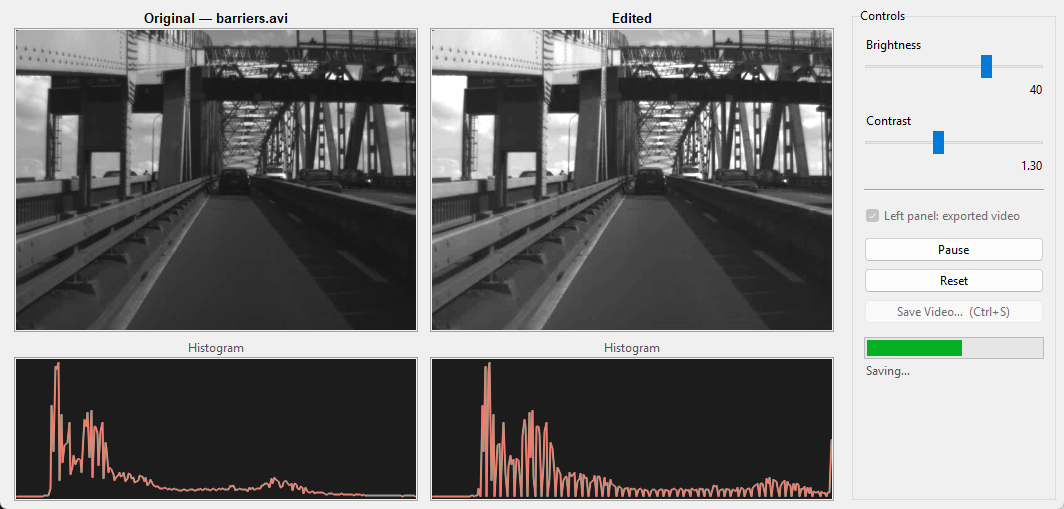
\includegraphics[width=\textwidth]{screenshot_save_progress.png}
        \caption{Export in progress}
        \label{fig:save-progress}
    \end{subfigure}
    \hfill
    \begin{subfigure}{0.48\linewidth}
        \centering
        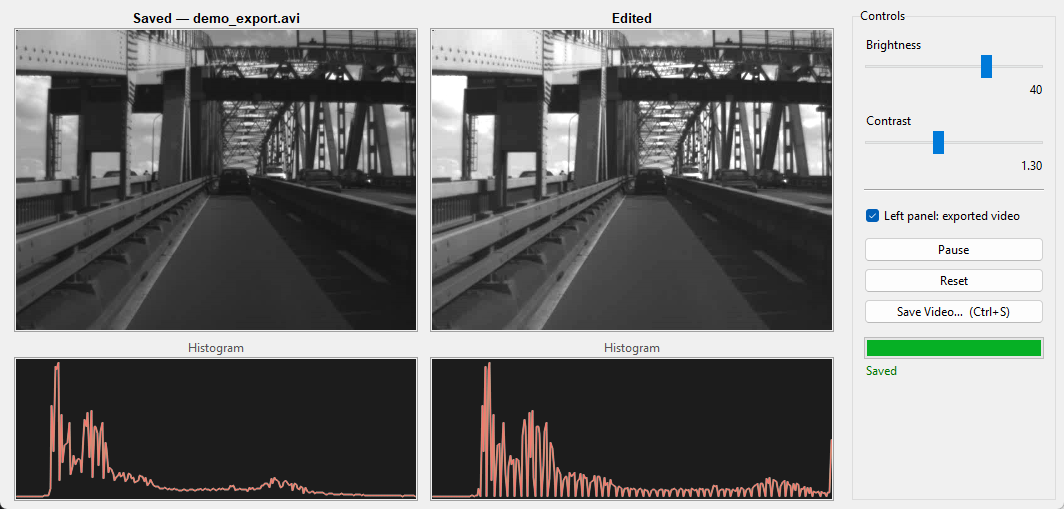
\includegraphics[width=\textwidth]{screenshot_save_done.png}
        \caption{Export complete}
        \label{fig:save-done}
    \end{subfigure}
    \caption[Save operation.]%
    {Saving with $\beta=40$, $\alpha=1.3$: (a) the ``Save Video\ldots''
    button disabled and the progress bar advancing while
    \texttt{\_save\_worker} re-encodes the source on a background
    thread; (b) after completion, the status reads ``Saved'' and the
    left panel automatically switches to play back the exported file
    (caption updates to ``Saved --- demo\_export.avi'').}
    \label{fig:save}
\end{figure}


%%%%%%%%%%%%%%%%%%%%%%%%%%%%%%%%%%%%%%%%%%%%%%%%%%%%%
\section{Settings Restored After Reload}
\label{sec:res-persist}
%%%%%%%%%%%%%%%%%%%%%%%%%%%%%%%%%%%%%%%%%%%%%%%%%%%%%

% Covers Task 8.
% TODO: before/after a restart -- same slider positions, same appearance
% in both windows.

\begin{figure}[H]
    \centering
    \begin{subfigure}{0.48\linewidth}
        \centering
        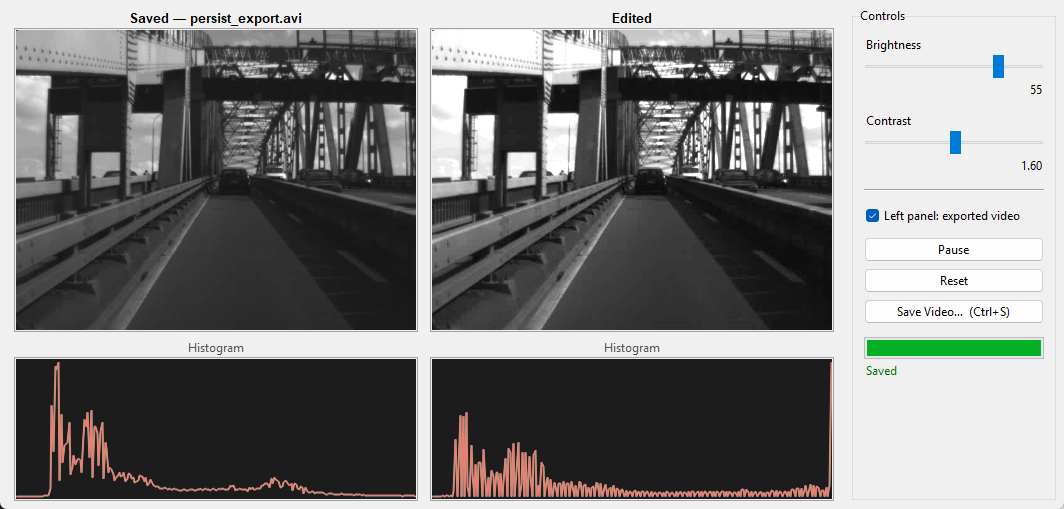
\includegraphics[width=\textwidth]{screenshot_persist_before.png}
        \caption{Before closing the program}
        \label{fig:persist-before}
    \end{subfigure}
    \hfill
    \begin{subfigure}{0.48\linewidth}
        \centering
        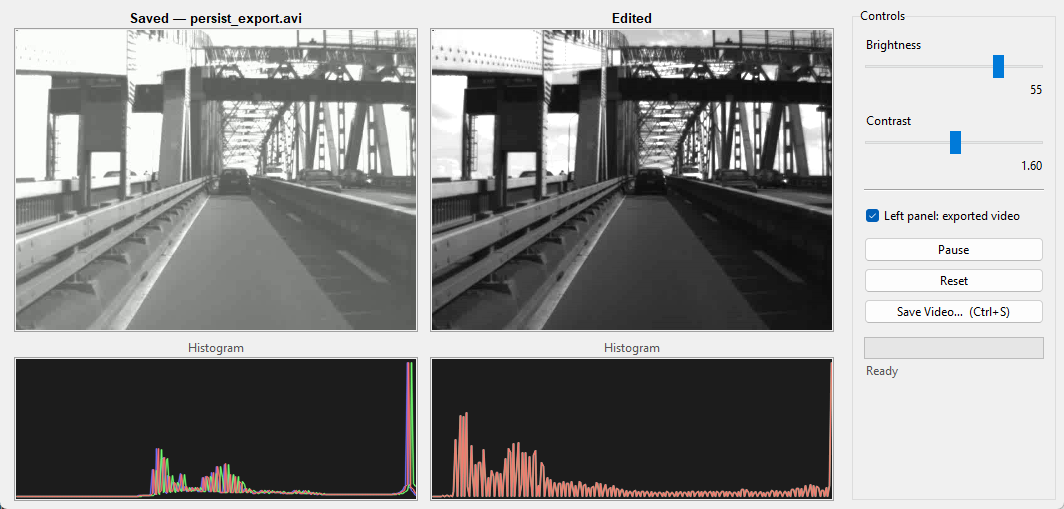
\includegraphics[width=\textwidth]{screenshot_persist_after.png}
        \caption{After restarting the program}
        \label{fig:persist-after}
    \end{subfigure}
    \caption[Settings restored on reload.]%
    {Brightness ($\beta=55$), contrast ($\alpha=1.6$), and the
    exported-video checkbox are all identical before closing (a) and
    immediately after a fresh launch (b), confirming that
    \texttt{settings.json} (Listing \ref{lst:task8-persist}) round-trips
    correctly.}
    \label{fig:persistence}
\end{figure}
